\documentclass{article}
\usepackage{tempora}
\usepackage{indentfirst}
\usepackage{tabularx}
\usepackage{caption}
\usepackage{graphicx}
\usepackage{longtable}
\usepackage{tabularx}
\usepackage{amsmath}
\usepackage{amsfonts}
\usepackage{floatrow}
\floatsetup[table]{capposition=top}
\makeatletter
\graphicspath{ {./images/} }
\renewcommand*\l@section{\@dottedtocline{1}{1.5em}{2.3em}}
\makeatother
\usepackage{float}
\usepackage[english, russian]{babel}
\begin{document}
  \textbf{Постановка задачи}.

  Решается задача поиска оптимального распределения функционала программного средства по плагинам для интеграции в плагинную систему с уменьшенем связности его компонентов. При этом существуют ограничения на общее число используемых плагинов и на распределение функционала по ним. Функционал описан в требованиях к программному средству и реализован в файлах исходного кода на языке программирования.

  \begin{figure}[H]
      \centering
      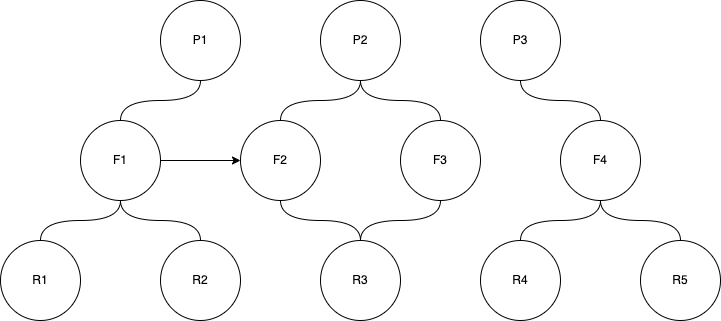
\includegraphics[width=1\textwidth]{Исходный граф.drawio}
      \caption{Граф $G$}
  \end{figure}

  Описание модели:
  \begin{itemize}
    \item Требования $R$ в количестве $n$ штук.
    \item Файлы исходного кода $F$ в количестве $m$ штук
    \item Плагины $P$ в количестве $k$ штук
    \item Требования трассируются на файлы исходного кода и образуется матрица связей $E_{rf} = m \times n$.
    \item Файлы исходного кода имеют друг на друга зависимости. Поэтому необходима матрица зависимостей $E_{ff} = m \times m$.
    \item Файлы исходного кода распределены по плагинам и образуется матрица связей $E_{fp} = k \times m$
  \end{itemize}

  Для указания необходимых в поставке требований модель принимает на вход вектор $R$ элементов. Элементы на позициях соответствующих индексам полезных требований равны $1$, бесполезных - $0$.

  Например: $R = \{R_1 = 1, R_2 = 0, ..., R_n = 1\}$.

  Необходимыми условиями трассируемости требований на файлы исходного кода является:
  \begin{itemize}
    \item каждое требование должно быть реализовано по меньшей мере в одном файле
    \item каждый файл реализует по меньшей мере одно требование
  \end{itemize}

  Эти условия можно записать в виде следующих ограничений:



  Это накладывает следующие ограничения на элементы матрицы трассируемости:
  \begin{itemize}
    \item если требование $i$ не трассируется на файл $j$ элемент $E_{fr_{00}} = 0$
    \item 
    \item $\bigtriangleup \not = 0$

  \end{itemize}

  Задача сводится к поиску оптимального распределения файлов по плагинам. Для поиска оптимального распределения можно использовать выборки поставляемых требований. Всего существует $2^n - 1$ возможных выборок поставляемых требований. Возможные комбинации удобно записать в виде таблицы:
  \begin{table}[H]
    \caption{Table 1}
    \begin{center}
      \begin{tabular}[H]{|c|c|c|c|c|}
         n  & n - 1 & ... &  2  &  1  \\
         \hline
         0  &   0   & ... &  0  &  1  \\
         0  &   0   & ... &  1  &  0  \\
         0  &   0   & ... &  1  &  1  \\
        ... &  ...  & ... & ... & ... \\
         0  &   1   & ... &  0  &  0  \\
         0  &   1   & ... &  0  &  1  \\
         0  &   1   & ... &  1  &  0  \\
         0  &   1   & ... &  1  &  1  \\
        ... &  ...  & ... & ... & ... \\
         1  &   0   & ... &  0  &  0  \\
         1  &   0   & ... &  0  &  1  \\
         1  &   0   & ... &  1  &  0  \\
         1  &   0   & ... &  1  &  1  \\
        ... &  ...  & ... & ... & ... \\
         1  &   1   & ... &  0  &  0  \\
         1  &   1   & ... &  0  &  1  \\
         1  &   1   & ... &  1  &  0  \\
         1  &   1   & ... &  1  &  1  \\
      \end{tabular}
    \end{center}
  \end{table}

\end{document}
